% REMEMBER: You must not plagiarise anything in your report. Be extremely careful.

\documentclass{l4proj}

   
%
% put any additional packages here
%

\begin{document}

%==============================================================================
%% METADATA
\title{Exploring 3D printing technologies for robotic grasping. }
\author{Adam Christie}
\date{September 14, 2019}

\maketitle

%==============================================================================
%% ABSTRACT
\begin{abstract}
  Every abstract follows a similar pattern. Motivate; set aims; describe work; explain results.
  \vskip 0.5em
  ``XYZ is bad. This project investigated ABC to determine if it was better. 
  ABC used XXX and YYY to implement ZZZ. This is particularly interesting as XXX and YYY have
  never been used together. It was found that  
  ABC was 20\% better than XYZ, though it caused rabies in half of subjects.''
\end{abstract}

%==============================================================================

% EDUCATION REUSE CONSENT FORM
% If you consent to your project being shown to future students for educational purposes
% then insert your name and the date below to sign the education use form that appears in the front of the document. 
% You must explicitly give consent if you wish to do so.
% If you sign, your project may be included in the Hall of Fame if it scores particularly highly.
%
% Please note that you are under no obligation to sign 
% this declaration, but doing so would help future students.
%
\def\consentname {Adam Christie} % your full name
\def\consentdate {20 March 2020} % the date you agree
%
\educationalconsent


%==============================================================================
\tableofcontents

%==============================================================================
%% Notes on formatting
%==============================================================================
% The first page, abstract and table of contents are numbered using Roman numerals and are not
% included in the page count. 
%
% From now on pages are numbered
% using Arabic numerals. Therefore, immediately after the first call to \chapter we need the call
% \pagenumbering{arabic} and this should be called once only in the document. 
%
% Do not alter the bibliography style.
%
% The first Chapter should then be on page 1. You are allowed 40 pages for a 40 credit project and 30 pages for a 
% 20 credit report. This includes everything numbered in Arabic numerals (excluding front matter) up
% to but excluding the appendices and bibliography.
%
% You must not alter text size (it is currently 10pt) or alter margins or spacing.
%
%
%==================================================================================================================================
%
% IMPORTANT
% The chapter headings here are **suggestions**. You don't have to follow this model if
% it doesn't fit your project. Every project should have an introduction and conclusion,
% however. 
%
%==================================================================================================================================
\chapter{Introduction}
% reset page numbering. Don't remove this!
\pagenumbering{arabic} 


To introduce this dissertation I believe it is important to first give some examples that highlight to us how applicable and important 3D printing is in today's world. Imagine engineers on a space station, trying to find some workaround to replace a broken end-effector on a robotic arm. Or a research and development team trying to quickly prototype their ideas. Or even a carpenter that wants to create a strong and precise jig that he can use to speed up his work. 

In all of these situations, 3D printing can potentially offer a way to quickly design reliable and accurate parts efficiently. This wide range of possible applications shows to me that there is potential to 3D printing that we do not currently utilise.  

When looking at robotics, from the high-end robots of BostonDynamics, to earth and space exploration, the technology can add not only safety, but in some cases a better way of life for people. Our one drawback of robotics is the expense, which we would be able to somewhat mitigate using 3D printing. In this chapter, I will outline the motivation for using 3D printing within robotics and will lay out a series of research goals that I will aim to complete during this project. 


\section{Motivation}
3D printing has slowly evolved from basic resin layering (Charles Hull 1983)[1], to the refined and precise printers that we know of today. As this technology has improved over the years its applications have spanned into all aspects of life and technology and it has quickly become a way to cheaply create prototypes and quick permanent solutions to problems. On the opposite end of the cost spectrum, we have robotics, with factory robotic arms costing anywhere between \$25,000 to 400,000 [2], or the University of Glasgow's Baxter which cost around £13,000 not including VAT and installation costs. So this is not something that the average person can afford.

Even at these high prices, researchers often find themselves at a disadvantage of only having a very limited selection of grippers to choose from and are often forced to compensate for the mechanical disadvantages of some designs with either highly specialised code or external systems[3]. 3D printing has brought us the ability to either quickly customise these designs to fit with specific needs, or to design the grippers from scratch. This becomes very attractive since a lot of designs and documentation are open source, meaning researches can pick and choose from a wide range of already existing designs.  

This is the basis of my dissertation. Are we able to find open-sourced 3D gripper designs, that we can take, modify if needed, print, program and run? This will show us how easy it can be for researchers to do the same, saving them a large amount of time and money. Another aspect I wish to explore is am I able to create generic code that works on very different gripper designs? This will show again how much time researchers can save by having one generic program that runs several grippers, rather than having to create new code for each one. 


\section{Aims and Goals}
The aim of this dissertation is to explore the benefits of 3D printing in robotics, specifically in robotic grippers. During this project, I will aim to:

\begin{itemize}
  \item
  Research a range of existing gripper designs and choose, from them, two that I believe will be the most appropriate to this project. This will involve finding grippers that have different opening and closing methods, different degrees of freedom and different geared mechanisms. This will also require research into what types of motors will be needed to power them. Some will require simpler 180$^{\circ}$ servomotors, while others will require more complex 360$^{\circ}$ motors that will need feedback to control.
  \item
  3D print the two chosen gripper designs. I will either use online and open-sourced STL files that I will get during research, or if these are not available, using CAD software I will try and replicate the design. While 3D printing I will have to ensure that all the correct calibrations are done before each print to ensure that the parts are as high quality as possible. These will have to be assembled and the motors will then be attached.
  \item
  Design and implement code that will give control of the grippers using an Arduino board that I will integrate using the ROS (Robotic Operating System) middleware. The designed code must be able to work on both designs meaning it can't be dependant on motor type, speed, or if it's a continuous motor or not. 
  \item
  Evaluate the performance of the grippers with user tests, tests on their ability to grip and hold objects, and by verifying that they both meet their requirements. This will need to be done with a range of objects of varying shapes, sizes and weights in order to stress test the capabilities of both grippers. 
\end{itemize}

By the end of these goals, we will hopefully be able to prove that not only is 3D printing a much cheaper way for robotics research to be done, but that it also provides us with grippers that are as useful as existing manufactured designs, and that can be programmed efficiently.



%==================================================================================================================================
\chapter{Background}
In this section I plan on researching each aspect of my project thoroughly, so that I can get a better understanding of what other people have already done in this field, what components and tools there are currently available to me, and what designs are currently available online. By conducting this research we are also able to identify the best parts and designs to use. This will involve current applications in 3D printing, including applications related to robotics, and a product overview, where we will look at gripper design, software frameworks and motors that we can utilise. 

\section{3D printing applications}
\subsection{Rapid Prototyping}
Until recently, prototyping required skilled tradesmen to produce accurate models, often taking weeks or months to go from detailed 2D hand-drawn designs to then producing the end model from this. 3D printing has given us a completely new outlook on prototyping, as we are now able to mock-up designs and print them on the same day, opening up windows in the manufacturing process for quick modifications and changes if necessary. D.T Pham states that the introduction of rapid prototyping could reduce production costs by up to 70\% and cut time to market by 90\%[4]. 

Pham's paper[4] gives us an outline of the many branches that come under rapid prototyping, the two main ones being material addition, also known as Additive Manufacturing, and material removal. There are even more subcategories under each, see figure2.1, but the majority of material addition processes are different types of 3D printing. Stereolithography (SLA) is one of the earliest versions of 3D printing, layering a photosensitive resin that reacts to UV light. Pham states that this is the most common technique used when rapid prototyping as it is fast, produces a good finish and is a well-proven system that is trusted with manufacturers. However, the resin used is toxic and is often brittle and mechanically weak once printed, making it unusable for many prototyping applications and not suitable for this project.

Fusion Deposition Modelling (FDM), another 3D printing additive manufacturing process, uses molten plastic, built up layer by layer to create the design. This process offers a range of materials to use, PLA, ABS, PETG and more, meaning that there are different materials for different needs. Most of these are robust and strong materials, not to mention that it is non-toxic and environmentally safe. Having this range can be very useful, especially when compared to SLA which only offers a small range, usually dependant on the manufacturer of the printer. This method is cheap and easy to use, CAD models simply need to be "Sliced" into a g-code format, so they can then be uploaded to an FDM printer. We then have our prototype ready any time from minutes to hours, depending on the size. This seems like it would be the most suitable method for this project and the fact that the university already has these printers available makes it even more attractive. 

\begin{figure}[!ht]
  \centering
  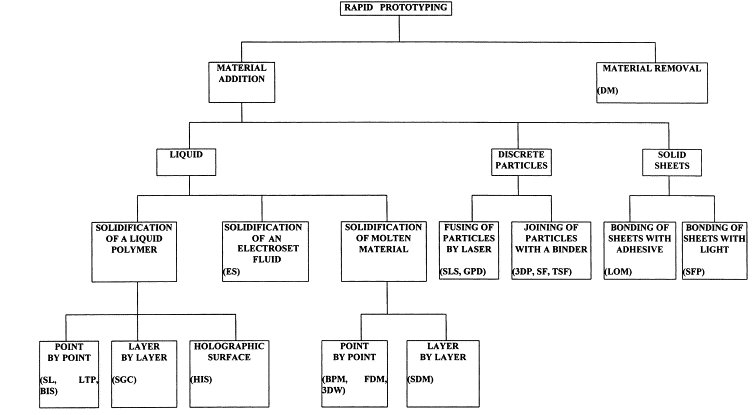
\includegraphics[width=0.9\linewidth]{images/rapidPrototyping.png}   

  \caption{Shows us a drop-down tree of the different types of rapid prototyping [4].}
\end{figure}


\subsection{Researchers \& Robotics}
Robotics can be incredibly expensive, for example, one of the robotic arms found at the University of Glasgow, the UR3, cost £13,000 not including VAT, which is already considered cheap. In contrast to this, lecturer Dr. Aragon Camarasa 3D printed a robotic arm similar to the UR3, costing him in total £500. This is a huge difference, giving researchers or developers a way to study robotics affordably. 

One very interesting application of 3D printing in robotics is Poppy[5]. Poppy is the world's first open-source 3D printed humanoid robot. It was originally being built in order to study the role of morphology (changing the shape of body parts) in sensorimeter control, however, until recently this was difficult as manufacturing processes were very expensive. By shifting the Poppy project to use 3D printing techniques, they were able to create a humanoid robot that they can explore new body shapes within a matter of days. This allowed the researching team to fully investigate how the morphology of the robot changed biped locomotion, meaning that they were able to produce a range of thigh designs that they could implement quickly and cheaply for investigations.

The research paper [3] gives some very good insight into the uses of 3D printing in robotic grippers. Whilst this paper is primarily focused on the design mechanisms of the gripper it does go into some detail on the uses and benefits of using 3D printing for robotic grippers. Here they use ABS plastic, due to its softness meaning that they could use simple dowels to fasten parts together. The paper states that most grippers in the industry currently fall into two categories, either simple and highly specialised, or general and extremely complicated. The high price often leads to researchers having to compensate for mechanical disadvantages with complex software. Perhaps, for example, the highly specialised part that has been purchased can't grip irregular objects without accurate feedback and intense software, whereas quickly 3D printing an under-actuated design that conforms to an object without feedback would likely be easier and more time-efficient. 

There is a wide range of possible uses for 3D printing in robotics that haven't been fully utilised yet, for example, NASA's Dextre[6]. This is a robotic arm, designed by Canada's space agency, currently located on the ISS. Dextre performs a wide variety of functions that previously would've involved dangerous spacewalks for the astronauts. It has a wide range of end-effectors and other equipment, such as cameras and lights, that allow it to do a range of jobs such as replacing batteries, testing equipment and even fixing electrical circuits[7]. But what would happen if one of its end-effectors broke? At this stage, the astronauts on the ISS would have to do this routine maintenance themselves, until the new parts arrive at the ISS. These cargo flights use the SpaceX Dragon spacecraft and their schedule times aren't evenly spaced, meaning the crews can go anywhere from days to months without getting new supplies[8]. Instead, the astronauts could 3D print the part, and use this until the cargo shipment arrived. This would minimise the risk put onto the astronauts as they would no longer have to pick up Dextre's routine duties. 


\section{Product Overview}

\subsection{Gripper Mechanisms}
Robots can have many different pieces of equipment attached to their arms, the end-effector is a generalising term that includes all devices that can be installed on to a robot wrist. This can include many different types of equipment, including welding torches, collision sensors, tool changers and of course, grippers. 

One main design choice for robotic grippers is how many degrees of freedom it will have. The textbook [9], describes DOF as the number of independent coordinates necessary for the movement of the gripper. So a gripper that has two jaws that move left and right would only have one degree of freedom. There are several basic types of gripper geometries, as described by Mouhammad Abomoharam and Alaa Hassan[10]. They state that the most basic type of these is a single degree of freedom design. These could come in many different shapes, however, such as-
\begin{itemize}
	\item
	A pair of geared jaws geared together and connected to a motor.
	\item
	A reciprocating lever gripper using rack and pinion based linear actuation. 
	\item
	Parallel jaws using four-bar linkage, similar to what is found in many pliers.
	\item 
	Multi-jawed grippers, such as three-fingered grippers 
\end{itemize}

Robotic gripper design is a very lengthy process that involves major design steps, such as kinematics design, dynamics design, thermal design and stiffness[11]. The research paper [11] describes the design of robots as an optimisation problem, in regards too geometric, kinematic and dynamic modeling. This modeling involves intense mathematical calculations that are above the scope of this project, but the gripper that the researchers decide on is a closed-loop mechanism with a single degree of freedom. So this design that they have decided to go for is one that can only move forward and backward and uses feedback in order to regulate itself, as it is a closed-loop system. See figure2.2 for design.

On top of degrees of freedom, another important design structure is whether to user full-actuated or under-actuated design. Under-actuated systems can be defined as systems in which the input, say a motor, cannot accelerate the robot in arbitrary directions[12]. This may seem like a negative feature, but in robotic grippers, an under-actuated design can be very useful, as they can allow the gripper to conform to the shape of the object that they're gripping. R. Ma[3] describes the design process to get adaptive under-actuation, in which they use a hybrid of a pulley system and a whiffle tree system (seen in figure2.3) to maximise the differential travel with the smallest gripped objects. Pulley systems can be very useful for getting the gripper to conform to objects however they can be fragile. If the motor continues to spin, once it's closed as far as it can, they can snap. This is undesirable when trying to design a robust and modular gripper to be used in a wide range of applications. 

Another interesting design is the four-bar and slider-crank design[10]. This gripper design consisted of four fingers, one of which acts as a driver finger and is driven by the motor. So as the motor spins and closes in the driver finger, the other three fingers are closed through the links shown in figure2.3b. Using one motor reduces the weight and cost of this design, whilst still retaining the optimal grasping stability that four fingers offer. A control circuit is also used on this design, using a stepper motor, transistors, and an ATmega8 microcontroller to control the gripper. This gripper uses a similar design to the four-bar linkage, with a bit more complexity, as shown in figure2.4.


\begin{figure}[!ht]
  \centering
  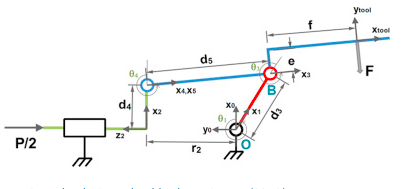
\includegraphics[width=0.75\linewidth]{images/image1.png}   
  \caption{Showing 1-DOF design, [11]}
  \label{fig:image1} 
\end{figure}

\begin{figure}[!ht]
  \centering
  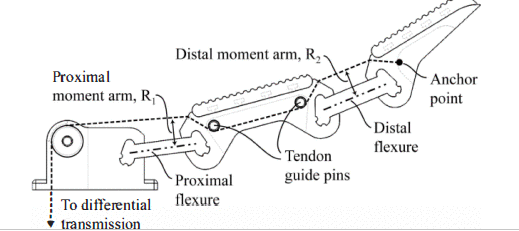
\includegraphics[width=0.75\linewidth]{images/image2.png}   
  \caption{Showing under-actuated finger design for conforming to objects, [3]}
\end{figure}

\begin{figure}[!ht]
  \centering
  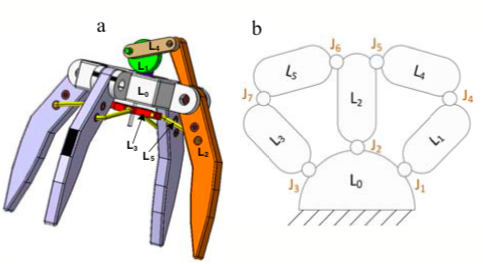
\includegraphics[width=0.75\linewidth]{images/fourfingered.png}   
  \caption{Showing four fingered bar and slider crank design, [10]}
\end{figure}


\subsection{Servo Motors}
A servo motor is a type of actuator that allows precise control of the motors position, velocity, and acceleration. Servos are found in many applications, from home electronics to cars and airplanes. Servos come in a variety of shapes and sizes, for the many different applications that they might have. Servos work by taking a small DC motor, that spins at a high RPM and uses a series of gears to increase the torque when needed. A positional sensor is placed on the final gear, which lets the circuit board know what position the motor is currently in. The circuit board takes in a signal from the user telling it what position to go to, decodes it and uses its knowledge from the current position to know how far to turn[13]. There are many types of motors that we could look at, such as DC or stepper motors, however servo motors offer very precise rotations and are often fast with high torque. Because of these benefits, they are generally thought of as the "Go-To" for robotics motors, making them perfect for this project. 
\\*Servo motors come in a wide range of designs and sizes, but there are three main ones to take a look at:
\begin{itemize}
	\item 
	\textbf{Positional rotation servo}: The shaft in a positional rotation servo rotates between 180$^{\circ}$, using a physical mechanism located in the gears to stop rotations outside of these limits. These are very often used in robotics as they offer very high precision positional control, making them an obvious choice for this project.
	
	\item
	\textbf{Continuous rotation servo}: These can continue in any direction indefinitely, offering open-loop speed control instead of the standard positional control. These started out as simply as hacked RC servos, removing the controller feedback so the motor position no longer mattered. Soon the industry recognised the need for these servo's so started producing them as well. These would be very useful for gripper designs that implemented a screw or gear and rack actuation, in which the servo will have to spin more than 180$^{\circ}$.
	\item
	\textbf{Linear servo}: This uses a gear and rack actuation, giving linear movement rather than rotational. These servos aren't used extensively and are generally more expensive than the other two. As they aren't used very often I don't think I will use one for this project. The aim is to try and create a gripper that will be widely used with parts that will be on hand to researchers. As these are hard to obtain and generally quite more expensive I don't think they would be useful. 
\end{itemize}

\subsection{DC Motors}
DC Motors are continuous rotation motors that work by converting DC electrical energy into mechanical energy, usually this means relying on the forces produced by a set of magnets and an electrical coil with a current flowing through it. 
\\There are two main types of DC motor: 
\begin{itemize}
	\item \textbf{Brush Motors}: Use contact brushes that connect with their commutator, commutator being the part that connects the rotating coils to the power supply. The brushes provide a current to the commutator that dictates what direction the shaft will rotate in. These motors are cheap and fairly easy to control, however require replacing due to the brushes wearing down.
	\item \textbf{Brushless Motors}: Typically use one or more permanent magnets in the core, and have a series of electromagnetic coils attached around the casing to spin it. While these are cheap and fairly long lasting, they require specialised regulators to ensure control. 
\end{itemize}


\subsection{Stepper Motors}
Stepper motors provide us with a simple and accurate open-looped system. They work by using two sets of teeth, as shown in image<<>>. There is the outside set, known as the stator teeth, have coils wrapped around them to provide electromagnetism, and the inside set, known as rotor teeth. By energising and de-energising sets of the stator teeth, we are able to spin the rotor teeth. These are simple motors that offer us high rotary position and provide us with a high torque at lower speeds and could prove very useful to this project. 

However most of these motors will only operate with a Driver module, as they require the logic for when to set its' stator poles to Low or High. These motors also require a very high current, some around 400mA but some larger ones can range right up to several amps[19]. 

\begin{figure}[!ht]
  \centering
  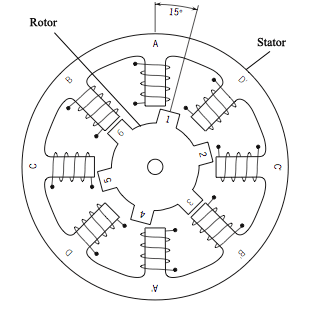
\includegraphics[width=0.4\linewidth]{images/stepMotor.png}   
  \caption{Stepper Motor internal drawing. These motors generally come with an unequal number of rotor and stator teeth so that only a pair can line up at any one time,}
\end{figure}

\subsection{ROS}
The Robotic Operating System is a middleware framework used to aid in writing the software for robotics[14]. ROS is able to utilise a very large collection of tools and libraries to simplify programming whilst still allowing for complex robotic operations. It was created by a wide range of experts and researches who contributed their time and resources to the core of ROS ideas and to the many packages that they now offer. As ROS was developed by many different researchers, all in different laboratories working on different robots, the main feature of ROS is that it is designed to be modular. This means that everyone from simple hobbyists, to large scale industrial systems, are able to use ROS to implement their systems for free. 

ROS provides many facilities, but I think what will be most useful for this project is the publisher/subscriber message passing capabilities. Messages are published onto topics, which the ROS nodes can use to exchange messages between each other. In the case of robotic grippers, these types of messages could be, if an open/close button is being pressed, feedback coming from the motor about its position or resistance to its rotation.

Because of its wide range of possible users, ROS has developed a very large, helpful community, offering over 22,000 wiki pages and a Q\&A website with over 13,000 questions asked that has a 70\% answer rate[15]. This makes ROS invaluable for this project. Not only is it beneficial to have a robotics platform that has such a wide range of packages for use, but for it to also have a helpful community makes any problem easier solved.




%==================================================================================================================================
\chapter{Requirements}
In this chapter we outline the requirements that the robotic grippers must fulfil in order to be considered successful and to achieve the goals we laid out in the introduction. This project was presented to me by Dr Gerardo Aragon Camarasa, a University of Glasgow lecturer, who wanted two robust and useful gripper designs that could be 3D Printed, and ran off the same program. We have had weekly meetings over the course of this project, slowly building up a solid list of requirements. This was done in a very agile way, where at each meeting it was discussed what stages the project was at and where we could take the requirements from there. 

\section{Problem Specification}
The following lays out the main specification and expectations for the final product. The goal of this project is that the gripper and software is easy to use, meaning that new users are able to pull from the open-source repository, set up the code and control the grippers. This would mean that in a real-world scenario researchers can quickly implement the code into either the  gripper designs we use in this project, or designs of their own. 

The functional requirements list the physical abilities the gripper needs to have as well as the tasks that the users should be able to perform on the gripper. Such as are they able to grasp objects of certain dimensions? Lift certain weights? Or read feedback from what they're gripping? The non-functional requirements list the constraints the program will have and its usability. These have then been laid out into a MoSCoW requirement structure.

\subsection{Functional Requirements}

\textbf{Must Have}
\begin{itemize}
	\item The grippers will open and close simply, using only two keys for control. By minimising the options for control we make this program easier to understand and therefore easier to modify by future users, to fit whatever purposes they have. 
	\item The motor will not push the gripper past its maximum or minimum constraints. This increases the safety of the system and decreases the likelihood that the gripper will break in use. 
	
\end{itemize}
\textbf{Should Have}
\begin{itemize}
	\item The grippers should be able to lift a weight of at least 0.5Kg, this will allow it to lift a wide variety of objects. This number is kept low as we are using servo motors, which aren't built for high torque (i.e. large weight) applications. 
	\item The motor should provide feedback to the software containing information on the grippers and their movement, such as velocity, present voltage or temperature. This will allow the software to calculate if an object is being gripped and whether it needs to stop the motor. 
\end{itemize}

\textbf{Could Have}
\begin{itemize}
	\item A "Hot-Swap" Tooling kit could be designed and created that fits with both gripper designs, that would allow quick swapping of each gripper on a robotic arm. This would allow users to switch between different gripper designs much more quickly, which would be beneficial to researchers. After discussions with my supervisor, we decided it would be best to ensure we had enough time first to do this. 
\end{itemize}


\subsection{Non-Functional Requirements}

\textbf{Must Have}
\begin{itemize}
	\item Users must be able to download and implement software in a reasonable time. This is important as it's quick usability is key to the whole project, and it was decided that as long as the average participant is able to implement it within 10 minutes. This should be adequate time for a user to clone our repository and perform the necessary setup to get the code to work. This is under the assumption that they already have installed the necessary ROS and Arduino software. 
	\item Must be usable without the need for a large amount of documentation, as this may put users off. A simple step-by-step guide on setting up is adequate, as well as some explanations on how the system works, in the case that users want to edit the code, should be enough
	\item Must use the same software for both grippers. This is important as we are trying to create a general API through which users can not only use the grippers from this project, but also gripper designs of their own. 
\end{itemize}

\textbf{Should Have}
\begin{itemize}
	\item The gripper should make its transition from closed to open and vice versa in an acceptable time. Within 7 seconds is acceptable, giving plenty of time for the grippers to perform their full movement. 
	\item The code should operate with minimal latency, meaning that the motor responds almost immediately to the input from the user. 
	\item The grippers must be able to grip objects of varying shapes.
\end{itemize}

\section{Changes to specification}
Will write if any changes come up once I'm finished. 

%==================================================================================================================================
\chapter{Design}
This chapter will give a high-level overview of this projects design process. It has been kept abstract to give the option of implementing it in a different language, using different frameworks, or with different hardware components. A more in-depth look into the project will be given in the Implementation section. 

\section{Hardware Design}

\subsection{Robotic Grippers}
When deciding on robotic gripper designs, it was established that two would be taken forward and used. This gave me the flexibility to find two different designs, that both had very different mechanisms of closing. Not only this, but it also allowed me to create two grippers that have advantages in different ways. 

\textbf{Gripper1}\\
The design of Gripper1, taken from an open-source 3D printing site [16], was chosen as it is commonly used in industry and because it gave us some very specific advantages. The shape of the gripper gives the robot the advantage of seeing what it is actually gripping, thanks to its flat design. This means that the cameras built on top of the robot would now be capable of viewing the object being gripped no matter what angle it was coming from, whereas previous robotic grippers used by Dr. Aragon-Camarasa meant the gripper had to come from the side.

The mechanism of the gripper is very similar to a rack and pinion, however, we have two racks working on one gear. Both racks are attached to the jaw and as they are on opposing sides of the gripper they turn in opposite directions to each other, creating a pincer movement. Whilst this design can not adapt or conform to the object it is gripping, it does have some advantages. As the jaws need to swing less than 180$^{\circ}$ we only need a simple servo motor to operate it, giving a cheap and simple alternative. It's simplicity also offers us less time to put it together and fewer parts that can break.

\textbf{Gripper2}\\
Gripper2 offers us a far more complex design, with 3 under-actuated fingers, each with 2 degrees of freedom. This gripper was designed by the Nazarbayev University and posted for public use on Wevolver[17]. These fingers work in a hybrid of both the under-actuated pulley design[3] and the four-bar crank design[10] discussed in Background. As the design is under-actuated, it allows the fingers to conform to whatever object it is gripping. This, along with having three fingers, gives researchers a large advantage when trying to grip irregular objects or spherical objects, that other, simpler grippers may struggle with. 

The mechanism used to turn the fingers is known as a worm and wheel composition, which is using a center screw (worm) in order to mesh with each of the gears (wheels) attached to the fingers. This design is very useful, as it is compact and allows for higher torque, but it will require +360$^{\circ}$ of motion in order to operate fully, meaning that we need a a motor that is not limited in its rotation (as the servo motor in Gripper 1), and can return positional eedback. 

\begin{figure}[!ht]
  \centering
  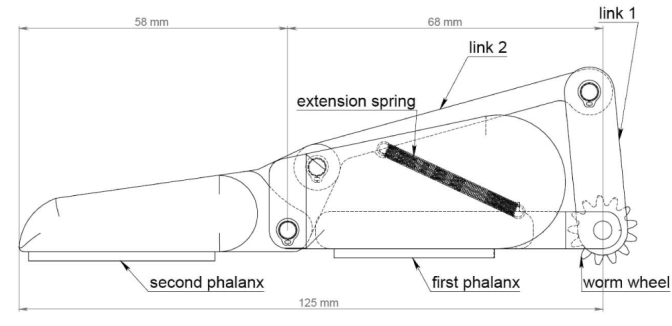
\includegraphics[width=0.75\linewidth]{images/gripper2_Finger.png}   
  \caption{Gripper2, 2-DOF under-actuated finger design. [17]}
  \label{fig:image1} 
\end{figure}

\subsection{Motors}
As stated, two different types of motors are needed for each of the gripper designs chosen. These motors can differ a lot on how they' are powered and controlled in a program.

\textbf{Servo Motors} are simpler motors that can rotate through 180$^{\circ}$. As these are so common and are widely used by hobbyists and researchers alike, they have been well integrated into systems such as Arduino and ROS. This means that controlling them is much easier and can be done by simply importing a few libraries. \textit{Servo.h}, for example, is an Arduino library that can be used to control the motor. This allows for simple commands to set the pin output and to write to the motor what position to travel to. It is important to note that when writing to servo motors we must provide them with an integer that correlates to the angle we want it to turn to. 

These motors have 3 wires, GND (ground line), VDD (voltage in line, to power the motor) and the control signal line, all of which must be connected to the Arduino to operate it. As servo motors only need around 5V to operate, we can connect it to the 5V output pin on the Arduino, then GND to the ground pin, and we cant set our data-out pin in the code, the data will then come through as a PWM signal from the Arduino. This is a pulse width modulation signal, essentially a square wave with varying high and low times to convey different information to the servo. The time the signal is high is known as the "Pulse Width" and determines what angle the servo travels to, the minimum pulse width for (1ms) example will turn the angle to its 0$^{\circ}$ point, whereas the maxiumum pulse width (2ms) would turn it to its 180$^{\circ}$ point. 

\textbf{Continuous Motors} are more complex and expensive than RC (Radio Controlled) servo motors, as previously said. These motors can provide feedback on load, voltage, torque, they can offer a range of rotational speeds and many give different modes of spinning. However, this feedback can be difficult to manage, as it very often requires external circuitry to switch the data line between read and write. The range of different modes can offer a lot of flexibility, allowing you to tailor the gripper to your specific needs, but for this project, I decided that either the Servo or Wheel mode would be of most use. Using Servo mode would offer similarities to the other motor, making it possibly easier to integrate the two codebases. However in the end the decision came from the design of the gripper that we use it with.  As our motor will have to complete several full rotations I decided that Wheel mode would have the most benefits, as it only requires the direction you wish to turn (clockwise or anti-clockwise) and the rotational speed. As the motor will have to spin through a much wider range this will offer more accuracy than having to guess at what angle to set the motor to turn to. 

Continuous motors, similar t RC servos, often have 3 wires, GND, VDD, and their data wire. However, these motors require a higher voltage than their servo cousins and so need a separate power source of 12V as the voltage provided by the Arduino is capped at 5V. While some Arduinos contain a voltage regulator and are able to take 12V, there are a few that cannot so it is best to plan for the general case. This leaves it as just the Data line being connected to the Arduino, although if the feedback is needed the data line will instead be connected to a Half-Duplex circuit, as described in the following section. 

\subsection{Half Duplex Circuit}
A half duplex system is one in which communication is available in both directions, but only one direction at a time. There are several real world examples of this kind of communication, such as "Walkie-Talkies" or an intercom. 

As our motor only has a single data-line, we must create a half duplex circuit that switches the direction of communication. This can be accomplished in many ways, with circuitry, with a separate micro-controller, or there are even some software libraries for the Arduino that are able to simulate Half Duplex communication.

Figure 4.2 shows a half-duplex circuit that can be created using a buffer chip, a few wires, a resistor and a breadboard. These are very basic components that most engineers would have on hand, and if not they are all very affordable. 

\begin{figure}[!ht]
  \centering
  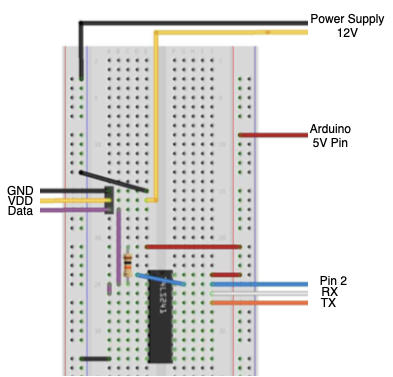
\includegraphics[width=0.75\linewidth]{images/half_dup_comm.png}   
  \caption{Basic Circuit for half duplex communication [18]}
  \label{fig:image1} 
\end{figure}

\section{Software Design}
\subsection{Publisher/Subscriber Architecture}
I decided early on that a publisher/subscriber architecture would be the most useful for this project, making the Arduino the subscriber and running a publisher on the computer. This is the easiest structure for passing information from distributed applications instantly so it was an obvious choice. 

\textbf{The publisher} will be created to read what keys on the keyboard are being used. Two keys will be selected as the controllers, one for opening and one for closing the grippers, for easy following we will now use keys "O" for open and "P" for close. We then must assign a numerical value to each of these keys, where one is greater than 0 and one less than (e.g. O=10 and P=-10). This allows us to perform different operations depending on which gripper we are using.\\
If we are using the continuous servo, then we simply publish the value associated with that key while it is being pressed, as long as the subscriber gets that value it will turn the servo that direction. If you then switch to the other key, the value (e.g. >0 now) is published and the subscriber will change the servo accordingly. \\
If we are using the regular servo, then we simply need to accumulate the value as long as the key is held and publish this total value continuously. This gives the servo a degree angle to turn to that continues to increase/decrease until the user releases the key. 

\textbf{The subscriber} will be the program stored on the Arduino. This means that it will have to perform the setup of the motors as well as listen for commands from the user. Continuous motors require setting up to set their ID, Baudrate, the maximum value of torque, etc. These must all be specified in the \textit{setup()} of the Arduino. When using the continuous motor a check will have to be performed if the key value is greater or less than 0 and spin the relevant direction, if we are using the servo it simply needs to write the key value to the servo. \\

\section{Technologies}
\subsection{Robotic Operating System}
ROS was chosen as my underlying framework due to the large number of tools and capabilities it had that I could utilise. Its publisher/subscriber pattern has been well tested on Arduinos and has documentation on how to use it, as well as some example programs to get new users familiar with it. As ROS offers many robot specific features, such as robot geometry libraries, robot description languages, a library for creating GUIs and even diagnostic tools, it is likely that researchers are already using it for their own robotics, so this aids in the integrability of the project. 

\subsection{Python}
Python was used to write the publisher script and was chosen between it and C++. Although C++ is more efficient, I decided on python as it was faster to program and much easier to read. The user must be able to understand what's being done in the code so that they can re-use it when needed in their research. Python is also an easy language to program in so it gave me a good launching point for the project. 

\subsection{Arduino} 
Arduinos are used extensively in research as they are an open-source microcontroller that are easily programmed and reprogrammed at any given time and are relatively cheap. They offer researchers and hobbyists alike a way to easily interact with their real world environment by using Arduino's sensor and actuator capabilities. Through the initial meeting with my supervisor, we discussed that using an Arduino was important for this project as it's so common for researchers to use.

\subsection{3D Printing and Computer-Aided Design}
A large portion of this project involves 3D printing components from a CAD design. Almost all of the components that make up the grippers need to be 3D printed, except for a couple of nuts and bolts, which means having a 3D printer on hand is vital. On top of this, a decision must be made on what plastic you use for the project, as this will have a large effect on the component's finish, strength, and brittleness. ±±±±±±±MUST ADD PLASTIC I USED AND 3D PRINTER USED±±±±±±±

%==================================================================================================================================
\chapter{Implementation 10/12}
This chapter describes the processes and steps taken to implement the functionality that was discussed in Chapter 4. This will go into greater detail than the previous chapters and aims to provide a process which others are able to take, use and even improve in their own work. 

\section{Resources Used}
\textbf{Ros Tutorials}: Were a very useful tool that provided me with the basic setup of my ROS system. Not only this, but the tutorials also provided a program called turtle_sim, which moved a turtle in the direction an arrow key was hit. Using this code I was then able to create a program that reacted to the gripper control keys. 

\textbf{Tic GUI}: Is a GUI provided by Polulu[20] and offers a full GUI for the Tic T500 Driver IC. This allowed me to configure my stepper motor before integrating it with the Arduino and ROS system. 

\textbf{Gripper Designs}: These were both open sourced and taken from locations already discussed and were used for both gripper designs, aside from some changes to Gripper2 that had to be made when changing motors. 
Discuss using a piece of example code from ROS. 


\section{System Overview}
What have I created, what can this do?
\subsection{Software Overview}
Discuss the teleop\_twist\_keyboard, need to change names of it:/. Discuss how it is to be changed depending on which motor is used. Then can discuss how there are two arduino code bases depending on which motor is being used, not in much detail as will have to dive in deeper later. 
Can talk about ROS launch. 
\subsection{Hardware Overview} 
General hardware setup, Pictures for both, talk about use of Arduino, Use of extra hardware such as the 3 motors used, USB2Dynamixel, a half duplex circuit, DynamixelShield, and the Tic T500. 



\section{Gripper 1}
Discuss design, insert pictures of fully assembled. Talk about applications of this type of gripper.
\subsection{Assembly}
Insert pics of individual pieces, discuss how the pieces are put together, the rubberised part for extra grip.
\subsection{Hardware}
Chance to discuss the motor in a bit of detail, pretty basic for servo motor. 
\subsection{Software}
Discuss what information is published to the subscriber and what it does with it. Why I chose this, why it seemed like the best option. 

\section{Gripper 2}
Discuss design, insert pictures of fully assembled. Talk about applications of this type of gripper.
\subsection{Assembly}
Pics of individual pieces/close-ups. How they've been put together, discuss how a new piece had to be created to fit the new motor.

\subsection{Hardware}
As discussed in previous chapters the hardware plan for the gripper2 was to use a Dynamixel Motor, with a Half-Duplex communication circuit. This motor was able to turn and function correctly to control the gripper, however due to an undetermined issue, I could not get feedback from the motor. This was a large issue as the reason an expensive motor was chosen was because it supposedly provided useful feedback. 

In order to check that it was not the fault of the motor I used a USB2Dynamixel from robotis, the same company that design the Dynamixel motors. This allowed me to plug the Dynamixel directly into a computer and use the DynamixelWizard software to view all the registers inside the Dynamixel and see how they changed with movement. Once it was clear the motor was not at fault research was conducted to determine the best way to retrieve feedback from the motor. Arduino shields seemed to be the biggest standout option, as certain types come with half-duplex logic built in. I decided that Robotis' own DynamixelShield would be the best purchase, as a component that is essentially made to work with our motor and they also provided open-source Arduino libraries to communicate with the shield and motor. 

Due to an issue while using these however a boot-loader error was hit and the motor was bricked. At this point time was running out and a solution had to be found quickly. During my initial background research I had reviewed other types of motors, such as DC motors and stepper motors so I decided that I would try and work with one of these. There was a stepper motor, 17HS13-0404D, and driver, Tic T500, at my disposal so I began work with it. 

Before starting with the Arduino some setup on the motor is required. Using open-source tooling from the company that provides the drivers, we can change the drive type, the max speed, max torque and see a range of values that the motor stores. I decided the best solution would be to set the mode to Analogue Speed controlled, so that I could provide a range of PWM signals from the Arduino to spin the motor. Once this was done the final circuit was configured with the Arduino as shown in image<<>>.


\subsection{Software}
Can discuss TicGUI and getting the motor setup. Also will have to discuss second Arduino program for this. 

\section{3D Printing}
Discuss the 3D printing, ensuring you recalibrate each time, wiping down surface areas, setting to relevant temperatures, feeding in plastic.
Creating new part for stepper motor. 

\section{Maintainability}
\subsection{Documentation}
%==================================================================================================================================
\chapter{Evaluation 10/11} 
How good is your solution? How well did you solve the general problem, and what evidence do you have to support that?

\section{Guidance}
\begin{itemize}
  \item
    Ask specific questions that address the general problem.
  \item
    Answer them with precise evidence (graphs, numbers, statistical
    analysis, qualitative analysis).
  \item
    Be fair and be scientific.
  \item
    The key thing is to show that you know how to evaluate your work, not
    that your work is the most amazing product ever.
\end{itemize}

\section{Evidence}
Make sure you present your evidence well. Use appropriate visualisations, reporting techniques and statistical analysis, as appropriate.

If you visualise, follow the basic rules, as illustrated in Figure \ref{fig:boxplot}:
\begin{itemize}
\item Label everything correctly (axis, title, units).
\item Caption thoroughly.
\item Reference in text.
\item \textbf{Include appropriate display of uncertainty (e.g. error bars, Box plot)}
\item Minimize clutter.
\end{itemize}

See the file \texttt{guide\_to\_visualising.pdf} for further information and guidance.

\begin{figure}
  \centering
  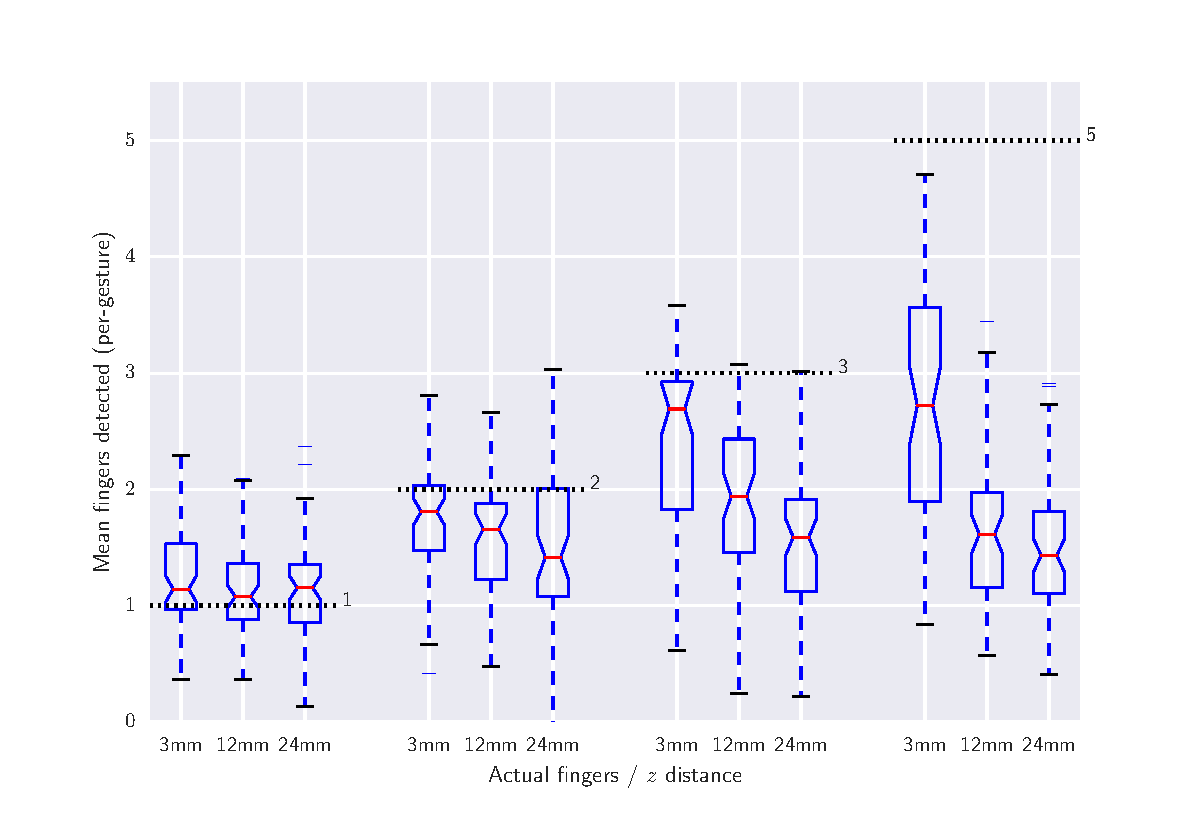
\includegraphics[width=1.0\linewidth]{images/boxplot_finger_distance.pdf}   

  \caption{Average number of fingers detected by the touch sensor at different heights above the surface, averaged over all gestures. Dashed lines indicate
  the true number of fingers present. The Box plots include bootstrapped uncertainty notches for the median. It is clear that the device is biased toward 
  undercounting fingers, particularly at higher $z$ distances.
  }

  % use the notation fig:name to cross reference a figure
  \label{fig:boxplot} 
\end{figure}


%==================================================================================================================================
\chapter{Conclusion 1/2}   
Summarise the whole project for a lazy reader who didn't read the rest (e.g. a prize-awarding committee).
\section{Guidance}
\begin{itemize}
  \item
    Summarise briefly and fairly.
  \item
    You should be addressing the general problem you introduced in the
    Introduction.     
  \item
    Include summary of concrete results (``the new compiler ran 2x
    faster'')
  \item
    Indicate what future work could be done, but remember: \textbf{you
    won't get credit for things you haven't done}.
\end{itemize}


///////////////////////////////////////////////////////////////////////////

\subsection{References and style guides}
There are many style guides on good English writing. You don't need to
read these, but they will improve how you write.

\begin{itemize}
  \item
  \emph{How to write a great research paper} \cite{Pey17} (\textbf{recommended}, even though you aren't writing a research paper)
  \item
  \emph{How to Write with Style} \cite{Von80}. Short and easy to read. Available online.
  \item
  \emph{Style: The Basics of Clarity and Grace} \cite{Wil09} A very popular modern English style guide.
\end{itemize}

\subsubsection{Citation styles}

\begin{itemize}
\item If you are referring to a reference as a noun, then cite it as: ``\citet{Orw68} discusses the role of language in political thought.''
\item If you are referring implicitly to references, use: ``There are many good books on writing \citep{Orw68, Wil09, Pin15}.''
\end{itemize}

There is a complete guide on good citation practice by Peter Coxhead available here: \url{http://www.cs.bham.ac.uk/~pxc/refs/index.html}. 
If you are unsure about how to cite online sources, please see this guide: \url{https://student.unsw.edu.au/how-do-i-cite-electronic-sources}.

%==================================================================================================================================
%
% 
%==================================================================================================================================
% APPENDICES  

\begin{appendices}

\chapter{Appendices}

Typical inclusions in the appendices are:

\begin{itemize}
\item
 Copies of ethics approvals (required if obtained)
\item
 Copies of questionnaires etc. used to gather data from subjects.
\item
 Extensive tables or figures that are too bulky to fit in the main body of
 the report, particularly ones that are repetitive and summarised in the body.

\item Outline of the source code (e.g. directory structure), or other architecture documentation like class diagrams.

\item User manuals, and any guides to starting/running the software.

\end{itemize}

\textbf{Don't include your source code in the appendices}. It will be
submitted separately.

\end{appendices}

%==================================================================================================================================
%  BIBLIOGRAPHY  

% The bibliography style is abbrvnat
% The bibliography always appears last, after the appendices.

\bibliographystyle{abbrvnat}


\bibliography{l4proj}
[1] 3D Systems, Our Story, https://uk.3dsystems.com/our-story

[2] https://insights.globalspec.com/article/4788/what-is-the-real-cost-of-an-industrial-robot-arm

[3] Raymond R. Ma, A modular, open-source 3D printed underactuated hand, https://ieeexplore.ieee.org/abstract/document/6630954

[4] D.T. Pham, A comparison of rapid prototyping technologies, 1998, https://www.sciencedirect.com/science/article/pii/S0890695597001375

[5] Matthieu Lapeyre, Poppy Project, https://hal.inria.fr/hal-01096338/document

[6] ISS Robotic Arm, https://www.nasa.gov/mission_pages/station/structure/elements/special-purpose-dextrous-manipulator/

[7] https://www.asc-csa.gc.ca/eng/iss/dextre/about.asp

[8] ISS Cargo delivery schedule, last visited 19/01/20, https://www.space.com/32286-space-calendar.html

[9] Robotics, 2010,, last visited 19/01/20, https://link-springer-com.ezproxy.lib.gla.ac.uk/content/pdf/10.1007%2F978-90-481-3776-3.pdf

[10] Mouhammad Abomoharam, Design of a single DOF gripper based on four-bar and slider-crank mechanism for educational purposes,, last visited 19/01/20, https://www-sciencedirect-com.ezproxy.lib.gla.ac.uk/science/article/pii/S221282711400732X?via%3Dihub

[11] Alaa Hassan, August 2017, Modeling and design optimization of a robot gripper mechanism,, last visited 19/01/20, https://www-sciencedirect-com.ezproxy.lib.gla.ac.uk/science/article/pii/S073658451630254X?via%3Dihub

[12] MIT, Fully Actuated vs. Underactuated Systems, last visited 19/01/20, https://ocw.mit.edu/courses/electrical-engineering-and-computer-science/6-832-underactuated-robotics-spring-2009/readings/MIT6_832s09_read_ch01.pdf

[13] Introduction to servo motors, AUTHOR??, last visited 19/01/20, https://www.sciencebuddies.org/science-fair-projects/references/introduction-to-servo-motors

[14] ROS, , last visited 19/01/20, https://www.ros.org/about-ros/

[15] ROS, last visited 19/01/20, https://www.ros.org/is-ros-for-me/

[16] Thingiverse- Gripper1 design, last visited 19/01/20, https://www.thingiverse.com/thing:1480408

[17] Wevolver, Gripper2 design, last visited 19/01/20, https://www.wevolver.com/wevolver.staff/3d.printed.robotic.gripper/master/blob/Assembly.wevolver

[18] Half-Duplex Circuit, last visited 08/02/20, https://github.com/zcshiner/Dynamixel_Serial/blob/master/Dynamixel%20Institution%20V2.pdf

[19] Stepper Motor Datasheet, last visited 18/02/20, https://www.oyostepper.com/images/upload/File/17HS13-0404D.pdf

[20] Polulu, Tic GUI, last visited 18/02/20, https://www.pololu.com/docs/0J71/all 

[c] https://www.ros.org/history/











\end{document}
